\documentclass[12pt,a4paper]{article}

\usepackage[utf8]{inputenc}
\usepackage{mathtools}
\usepackage{amssymb}
\usepackage{ntheorem}
\usepackage[framemethod=TikZ]{mdframed}
\usepackage{amsmath}
\usepackage[hidelinks]{hyperref}
\usepackage{cleveref}
\usepackage[most]{tcolorbox}
\usepackage{fancyhdr}
\usepackage{lastpage}
\usepackage{geometry}
\usepackage{graphicx}
\usepackage{float} 
\usepackage{subfigure} 
\usepackage{arydshln}
\usepackage{multicol}
\usepackage{url}
\usepackage{setspace}
\usepackage[T1]{fontenc}
\usepackage{mathptmx}
\usepackage{framed}
\usepackage{xcolor}
\usepackage{listings}
\usepackage{chemfig}
\usepackage{tikz}
\usepackage{pifont}



\geometry{a4paper, left=2cm, right=2cm, bottom=2cm, top=2cm}

\pagestyle{fancy}
\fancyhead{}
\fancyhead[L]{\leftmark}
\fancyhead[R]{\rightmark}
\fancyfoot{}
\fancyfoot[C]{\thepage}
%\renewcommand{\headrulewidth}{0pt}
\renewcommand{\footrulewidth}{0pt}

\definecolor{blue}{rgb}{0,0.45,1.14}
\definecolor{red}{rgb}{0.77,0.12,0.23}
\definecolor{grey}{rgb}{0.49,0.38,0.29}
\definecolor{green}{rgb}{0,0.42,0.24}
\definecolor{orange}{rgb}{2.07,0.69,0.32}

\theorembodyfont{\upshape}
\theoremseparator{.}
\newtheorem{thm}{Theorem}[subsection]
\newtheorem{df}{Definition}[subsection]
\newtheorem{eg}{Example}[subsection]
\newenvironment*{sol}{\indent\textbf{Solution. }}{\hfill{$\square$}\par}
\newtheorem*{rmk}{\indent Remark}
\newenvironment*{prf}{\indent\textbf{\textit{Proof. }}}{\hfill $\blacksquare$\par}
\newtheorem*{ext}{\indent Extension}

\linespread{1.25}


\title{Emory University\\\textbf{MATH 211 - Advanced Calculus (Multivariable) Learning Notes}}
\author{Jiuru Lyu}
\date{\today}

\linespread{1.22}

\def\Z{{\mathbb{Z}}}
\def\R{{\mathbb{R}}}
\def\C{{\mathbb{C}}}
\def\Q{{\mathbb{Q}}}
\def\E{{\mathbb{E}}}
\def\d{{\mathrm{d}}}
\def\i{{\mathrm{i}}}
\def\RE{{\mathrm{Re}}}
\def\IM{{\mathrm{Im}}}
\def\Arg{{\mathrm{Arg}}}
\def\cis{\mathrm{cis}}
\def\Proj{\mathrm{Proj}}
\def\qed{\rightline{$\blacksquare$}}
\def\ddx{\frac{\d}{\d x}}
\def\dydx{\frac{\d y}{\d x}}
\def\dx{\d x}
\def\vecx{\vec{x}}
\def\vecy{\vec{y}}
\def\vecv{\vec{v}}
\def\vecw{\vec{w}}
\def\vecu{\vec{u}}
\def\veca{\vec{a}}
\def\vecb{\vec{b}}
\def\vecc{\vec{c}}
\def\vece{\boldsymbol{\textbf{e}}}
\def\veci{\boldsymbol{\textbf{i}}}
\def\vecj{\boldsymbol{\textbf{j}}}
\def\veck{\boldsymbol{\textbf{k}}}
\def\DNE{\mathrm{D.N.E.}}
\def\LI{\mathrm{L.I.}}

\begin{document}
\maketitle
\tableofcontents
\newpage

\section*{Preface}
These is my personal notes for Emory University MATH 211 Advanced Calculus (Multivariable Calculus) course. 

After mastering Calculus I (which covers contents concerning limits, differentiation, and basic integration) and Calculus II (which includes integration techniques and series), this course focuses on multivariable calculus, including vectors, multivariable functions, partial derivatives, optimization, multiple integrations, vector and scalar fields, Green’s and Stokes’ theorems, and the divergence theorem. The book used for this course is \textit{Multivariable Calculus, 8th Edition} by James Stewart. 

Throughout this personal note, I use different formats to differentiate different contents, including definitions, theorems, proofs, examples, extensions, and remarks. To be more specific: 
\begin{df}[Terminology]
    This is a \textbf{definition}.	
\end{df}
\begin{thm}[Theorem Name]
    This is a \textbf{theorem}.	
\end{thm}
\begin{eg}
    This is  an \textbf{example}. 
\end{eg}

\begin{sol}
    This is the \textit{answer} part of an \textbf{example}. 
\end{sol}
\begin{rmk}
	This is a \textbf{remark} of a definition, theorem, example, or proof. 
\end{rmk}

\begin{prf}
	This is a \textbf{proof} of a theorem. 
\end{prf}
\begin{ext}
	This is a \textbf{extension} of a theorem, proof, or example. 	
\end{ext}
To better ace this course, it is recommended to do more questions than provided as examples under each section. Although each example is distinctive and representative, more questions and practice is still needed to deepen the understanding of this course. 

Even though I put efforts into making as few flaws as possible when encoding these learning notes, some errors may still exist in this note. If you find any, please contact me via email: \url{lvjiuru@hotmail.com}. 

I hope you will find my notes helpful when learning Multivariable Calculus.

\rightline{Cheers,}
\rightline{Jiuru Lyu}

\newpage
\section{Vectors and Geometry of Space}
\subsection{Three Dimensional Coordinate System}
\begin{df}[Coordinate System]
	A \textbf{coordinate system} is a system that uses coordinate of a point to uniquely determine the position of the point in the space or plane.	
\end{df}
The Cartesian coordinate system is defined in different dimensions.
\begin{df}[One Dimensional Cartesian System]
	\textbf{One Dimensional Cartesian System} is a straight line with a fixed point as the origin and positive and negative directions.
	\begin{rmk}
		The one dimensional cartesian system is the number line: 
		\begin{center}
		\tikzset{every picture/.style={line width=0.75pt}}	
		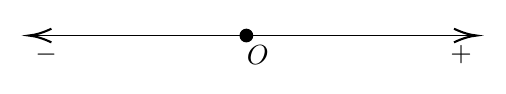
\begin{tikzpicture}[x=0.75pt,y=0.75pt,yscale=-1,xscale=1]
		\draw    (150,111) -- (361.83,111) ;
		\draw [shift={(363.83,111)}, rotate = 180] [color={rgb, 255:red, 0; green, 0; blue, 0 }  ][line width=0.75]    (10.93,-3.29) .. controls (6.95,-1.4) and (3.31,-0.3) .. (0,0) .. controls (3.31,0.3) and (6.95,1.4) .. (10.93,3.29)   ;
		\draw [shift={(148,111)}, rotate = 0] [color={rgb, 255:red, 0; green, 0; blue, 0 }  ][line width=0.75]    (10.93,-3.29) .. controls (6.95,-1.4) and (3.31,-0.3) .. (0,0) .. controls (3.31,0.3) and (6.95,1.4) .. (10.93,3.29)   ;
		\draw  [fill={rgb, 255:red, 0; green, 0; blue, 0 }  ,fill opacity=1 ] (249.83,111) .. controls (249.83,109.32) and (251.19,107.96) .. (252.87,107.96) .. controls (254.55,107.96) and (255.91,109.32) .. (255.91,111) .. controls (255.91,112.68) and (254.55,114.04) .. (252.87,114.04) .. controls (251.19,114.04) and (249.83,112.68) .. (249.83,111) -- cycle ;
		\draw (150,114.4) node [anchor=north west][inner sep=0.75pt]    {$-$};
		\draw (349.83,114.4) node [anchor=north west][inner sep=0.75pt]    {$+$};
		\draw (251.83,114.4) node [anchor=north west][inner sep=0.75pt]    {$O$};
		\end{tikzpicture}	
		\end{center}
	\end{rmk}
\end{df}
Any point in the one dimensional Cartesian system corresponds to a number $\in\R$ and any number $\in\R$ has a location on the line.
The two dimensional Cartesian system is the regular coordinate system. 
\begin{center}
\tikzset{every picture/.style={line width=0.75pt}}      
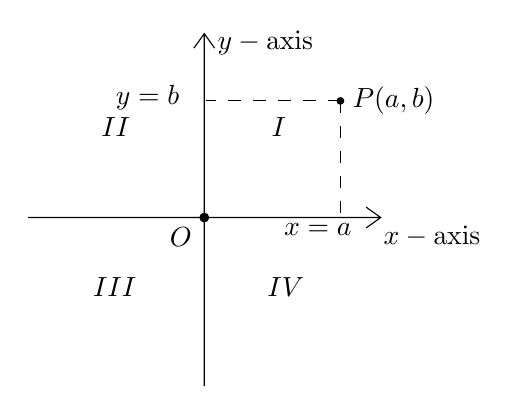
\begin{tikzpicture}[x=0.75pt,y=0.75pt,yscale=-1,xscale=1]
\draw  (50,146.61) -- (219.83,146.61)(134.83,58) -- (134.83,227.83) (212.83,141.61) -- (219.83,146.61) -- (212.83,151.61) (129.83,65) -- (134.83,58) -- (139.83,65)  ;
\draw  [fill={rgb, 255:red, 0; green, 0; blue, 0 }  ,fill opacity=1 ] (198.83,90.41) .. controls (198.83,89.54) and (199.54,88.83) .. (200.41,88.83) .. controls (201.29,88.83) and (202,89.54) .. (202,90.41) .. controls (202,91.29) and (201.29,92) .. (200.41,92) .. controls (199.54,92) and (198.83,91.29) .. (198.83,90.41) -- cycle ;
\draw  [fill={rgb, 255:red, 0; green, 0; blue, 0 }  ,fill opacity=1 ] (132.74,146.61) .. controls (132.74,145.45) and (133.68,144.52) .. (134.83,144.52) .. controls (135.98,144.52) and (136.91,145.45) .. (136.91,146.61) .. controls (136.91,147.76) and (135.98,148.69) .. (134.83,148.69) .. controls (133.68,148.69) and (132.74,147.76) .. (132.74,146.61) -- cycle ;
\draw  [dash pattern={on 4.5pt off 4.5pt}]  (200.41,90.41) -- (200.41,146.61) ;
\draw  [dash pattern={on 4.5pt off 4.5pt}]  (200.41,90.41) -- (135.83,90.41) ;
\draw (166,97.4) node [anchor=north west][inner sep=0.75pt]    {$I$};
\draw (84,97.4) node [anchor=north west][inner sep=0.75pt]    {$II$};
\draw (80,174.4) node [anchor=north west][inner sep=0.75pt]    {$III$};
\draw (164,174.4) node [anchor=north west][inner sep=0.75pt]    {$IV$};
\draw (220,149.4) node [anchor=north west][inner sep=0.75pt]    {$x-\text{axis}$};
\draw (140,55.4) node [anchor=north west][inner sep=0.75pt]    {$y-\text{axis}$};
\draw (205,82.4) node [anchor=north west][inner sep=0.75pt]    {$P( a,b)$};
\draw (117,150.4) node [anchor=north west][inner sep=0.75pt]    {$O$};
\draw (172,148.4) node [anchor=north west][inner sep=0.75pt]    {$x=a$};
\draw (91,81.4) node [anchor=north west][inner sep=0.75pt]    {$y=b$};
\end{tikzpicture}	
\end{center}
The three dimensional Cartesian system includes three perpendicular axes. 
\begin{center}
\tikzset{every picture/.style={line width=0.75pt}}
\begin{tikzpicture}[x=0.75pt,y=0.75pt,yscale=-1,xscale=1]
\draw  (125.83,146.62) -- (219.83,146.62)(135.14,58) -- (135.14,155.06) (212.83,141.62) -- (219.83,146.62) -- (212.83,151.62) (130.14,65) -- (135.14,58) -- (140.14,65)  ;
\draw  [fill={rgb, 255:red, 0; green, 0; blue, 0 }  ,fill opacity=1 ] (132.74,146.61) .. controls (132.74,145.45) and (133.68,144.52) .. (134.83,144.52) .. controls (135.98,144.52) and (136.91,145.45) .. (136.91,146.61) .. controls (136.91,147.76) and (135.98,148.69) .. (134.83,148.69) .. controls (133.68,148.69) and (132.74,147.76) .. (132.74,146.61) -- cycle ;
\draw    (134.83,146.61) -- (72.36,198.78) ;
\draw [shift={(70.83,200.06)}, rotate = 320.13] [color={rgb, 255:red, 0; green, 0; blue, 0 }  ][line width=0.75]    (10.93,-3.29) .. controls (6.95,-1.4) and (3.31,-0.3) .. (0,0) .. controls (3.31,0.3) and (6.95,1.4) .. (10.93,3.29)   ;
\draw (221,149.4) node [anchor=north west][inner sep=0.75pt]    {$y$};
\draw (140,55.4) node [anchor=north west][inner sep=0.75pt]    {$z$};
\draw (134.74,150.01) node [anchor=north west][inner sep=0.75pt]    {$O$};
\draw (72.83,203.46) node [anchor=north west][inner sep=0.75pt]    {$x$};
\end{tikzpicture}	
\end{center}
\begin{df}[Octant]
	A \textbf{Octant} is one of the eight divisions of the three dimensional coordinate system.	
\end{df}
\begin{df}[Hyperplane]
The hyperplane of $y=2$ is given as below: 
	\begin{center}
	\tikzset{every picture/.style={line width=0.75pt}}
	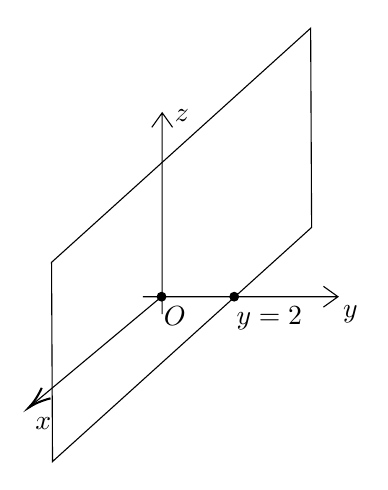
\begin{tikzpicture}[x=0.75pt,y=0.75pt,yscale=-1,xscale=1]
	\draw  (125.83,146.62) -- (219.83,146.62)(135.14,58) -- (135.14,155.06) (212.83,141.62) -- (219.83,146.62) -- (212.83,151.62) (130.14,65) -- (135.14,58) -- (140.14,65)  ;
	\draw  [fill={rgb, 255:red, 0; green, 0; blue, 0 }  ,fill opacity=1 ] (132.74,146.61) .. controls (132.74,145.45) and (133.68,144.52) .. (134.83,144.52) .. controls (135.98,144.52) and (136.91,145.45) .. (136.91,146.61) .. controls (136.91,147.76) and (135.98,148.69) .. (134.83,148.69) .. controls (133.68,148.69) and (132.74,147.76) .. (132.74,146.61) -- cycle ;
	\draw    (134.83,146.61) -- (72.36,198.78) ;
	\draw [shift={(70.83,200.06)}, rotate = 320.13] [color={rgb, 255:red, 0; green, 0; blue, 0 }  ][line width=0.75]    (10.93,-3.29) .. controls (6.95,-1.4) and (3.31,-0.3) .. (0,0) .. controls (3.31,0.3) and (6.95,1.4) .. (10.93,3.29)   ;
	\draw   (206.66,17.26) -- (207.13,113.23) -- (82.3,226.03) -- (81.83,130.06) -- cycle ;
	\draw  [fill={rgb, 255:red, 0; green, 0; blue, 0 }  ,fill opacity=1 ] (167.74,146.61) .. controls (167.74,145.45) and (168.68,144.52) .. (169.83,144.52) .. controls (170.98,144.52) and (171.91,145.45) .. (171.91,146.61) .. controls (171.91,147.76) and (170.98,148.69) .. (169.83,148.69) .. controls (168.68,148.69) and (167.74,147.76) .. (167.74,146.61) -- cycle ;
	\draw (221,149.4) node [anchor=north west][inner sep=0.75pt]    {$y$};
	\draw (140,55.4) node [anchor=north west][inner sep=0.75pt]    {$z$};
	\draw (134.74,150.01) node [anchor=north west][inner sep=0.75pt]    {$O$};
	\draw (72.83,203.46) node [anchor=north west][inner sep=0.75pt]    {$x$};
	\draw (169.74,150.01) node [anchor=north west][inner sep=0.75pt]    {$y=2$};
	\end{tikzpicture}
	\end{center}
	
	Specially: 
	\begin{center}
	\tikzset{every picture/.style={line width=0.75pt}}
	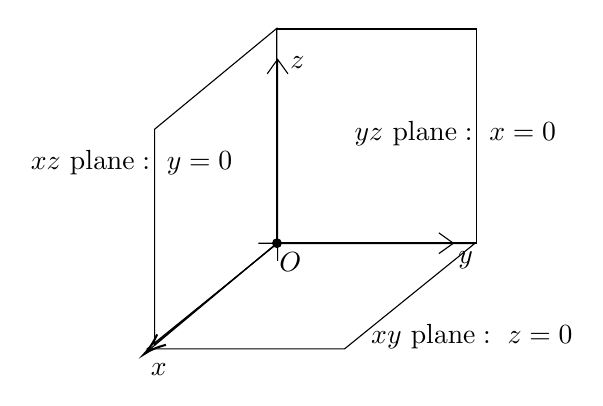
\begin{tikzpicture}[x=0.75pt,y=0.75pt,yscale=-1,xscale=1]
	\draw  (125.83,146.62) -- (219.83,146.62)(135.14,58) -- (135.14,155.06) (212.83,141.62) -- (219.83,146.62) -- (212.83,151.62) (130.14,65) -- (135.14,58) -- (140.14,65)  ;
	\draw  [fill={rgb, 255:red, 0; green, 0; blue, 0 }  ,fill opacity=1 ] (132.74,146.61) .. controls (132.74,145.45) and (133.68,144.52) .. (134.83,144.52) .. controls (135.98,144.52) and (136.91,145.45) .. (136.91,146.61) .. controls (136.91,147.76) and (135.98,148.69) .. (134.83,148.69) .. controls (133.68,148.69) and (132.74,147.76) .. (132.74,146.61) -- cycle ;
	\draw    (134.83,146.61) -- (72.36,198.78) ;
	\draw [shift={(70.83,200.06)}, rotate = 320.13] [color={rgb, 255:red, 0; green, 0; blue, 0 }  ][line width=0.75]    (10.93,-3.29) .. controls (6.95,-1.4) and (3.31,-0.3) .. (0,0) .. controls (3.31,0.3) and (6.95,1.4) .. (10.93,3.29)   ;
	\draw   (134.99,146.79) -- (230.08,146.79) -- (167.39,197.52) -- (72.3,197.52) -- cycle ;
	\draw   (134.83,43.03) -- (134.83,146.61) -- (75.88,195.27) -- (75.88,91.7) -- cycle ;
	\draw   (134.83,43.42) -- (230.83,43.42) -- (230.83,146.52) -- (134.83,146.52) -- cycle ;
	\draw (221,149.4) node [anchor=north west][inner sep=0.75pt]    {$y$};
	\draw (140,55.4) node [anchor=north west][inner sep=0.75pt]    {$z$};
	\draw (134.74,150.01) node [anchor=north west][inner sep=0.75pt]    {$O$};
	\draw (72.83,203.46) node [anchor=north west][inner sep=0.75pt]    {$x$};
	\draw (179,184.4) node [anchor=north west][inner sep=0.75pt]    {$xy\text{ plane} :\ z=0$};
	\draw (15,100.4) node [anchor=north west][inner sep=0.75pt]    {$xz\text{ plane} :\ y=0$};
	\draw (171,86.4) node [anchor=north west][inner sep=0.75pt]    {$yz\text{ plane} :\ x=0$};
	\end{tikzpicture}
	\end{center}
\end{df}
\begin{df}[Points in the Three Dimensional System]
	$P(a,b,c)$ indicates the intersection of the three hyperplanes: $x=a$, $y=b$, and $z=c$.	
	\begin{center}
	\tikzset{every picture/.style={line width=0.75pt}}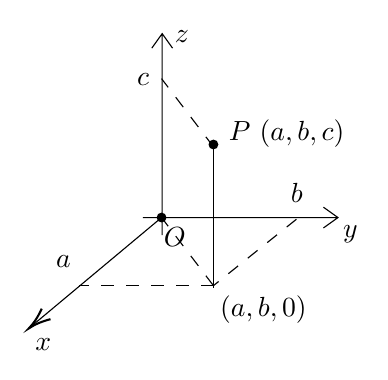
\begin{tikzpicture}[x=0.75pt,y=0.75pt,yscale=-1,xscale=1]
	\draw  (125.83,146.62) -- (219.83,146.62)(135.14,58) -- (135.14,155.06) (212.83,141.62) -- (219.83,146.62) -- (212.83,151.62) (130.14,65) -- (135.14,58) -- (140.14,65)  ;
	\draw  [fill={rgb, 255:red, 0; green, 0; blue, 0 }  ,fill opacity=1 ] (132.74,146.61) .. controls (132.74,145.45) and (133.68,144.52) .. (134.83,144.52) .. controls (135.98,144.52) and (136.91,145.45) .. (136.91,146.61) .. controls (136.91,147.76) and (135.98,148.69) .. (134.83,148.69) .. controls (133.68,148.69) and (132.74,147.76) .. (132.74,146.61) -- cycle ;
	\draw    (134.83,146.61) -- (72.36,198.78) ;
	\draw [shift={(70.83,200.06)}, rotate = 320.13] [color={rgb, 255:red, 0; green, 0; blue, 0 }  ][line width=0.75]    (10.93,-3.29) .. controls (6.95,-1.4) and (3.31,-0.3) .. (0,0) .. controls (3.31,0.3) and (6.95,1.4) .. (10.93,3.29)   ;
	\draw  [fill={rgb, 255:red, 0; green, 0; blue, 0 }  ,fill opacity=1 ] (157.74,111.42) .. controls (157.74,110.27) and (158.68,109.34) .. (159.83,109.34) .. controls (160.98,109.34) and (161.91,110.27) .. (161.91,111.42) .. controls (161.91,112.58) and (160.98,113.51) .. (159.83,113.51) .. controls (158.68,113.51) and (157.74,112.58) .. (157.74,111.42) -- cycle ;
	\draw    (159.83,111.42) -- (159.83,180.42) ;
	\draw  [dash pattern={on 4.5pt off 4.5pt}]  (199.83,147.42) -- (159.83,179.42) ;
	\draw  [dash pattern={on 4.5pt off 4.5pt}]  (159.83,179.42) -- (94.83,179.42) ;
	\draw  [dash pattern={on 4.5pt off 4.5pt}]  (159.83,179.42) -- (134.83,146.61) ;
	\draw  [dash pattern={on 4.5pt off 4.5pt}]  (159.83,112.51) -- (134.83,79.69) ;
	\draw (221,149.4) node [anchor=north west][inner sep=0.75pt]    {$y$};
	\draw (140,55.4) node [anchor=north west][inner sep=0.75pt]    {$z$};
	\draw (134.74,150.01) node [anchor=north west][inner sep=0.75pt]    {$O$};
	\draw (72.83,203.46) node [anchor=north west][inner sep=0.75pt]    {$x$};
	\draw (166,98.4) node [anchor=north west][inner sep=0.75pt]    {$P\ ( a,b,c)$};
	\draw (161.83,182.82) node [anchor=north west][inner sep=0.75pt]    {$( a,b,0)$};
	\draw (82.83,163.82) node [anchor=north west][inner sep=0.75pt]    {$a$};
	\draw (195.83,128.82) node [anchor=north west][inner sep=0.75pt]    {$b$};
	\draw (121.83,75.82) node [anchor=north west][inner sep=0.75pt]    {$c$};
	\end{tikzpicture}
	\end{center}
\end{df}
For spaces in the higher dimension, we understand them via the Cartesian product. 
\begin{df}[Cartesian Product]
	\[\R\times\R\times\cdots\times\R=\{(x_1,\cdots,x_n)|x_i\in\R\forall i=1,\cdots,n\}\] is the set of all $n$-tuples of real numbers and is denoted by $\R^n$.
\end{df}
\begin{eg}
		$(3,4,5)\in\R^3$ is 3 dimensional. $(3,4,5,6)\in\R^4$ is 4 dimensional.	
\end{eg}
\begin{eg}
	Which point(s) $(x,y,z)$ satisfies the equations \[x^2+y^2=1\quad\text{and}\quad x=3? \]	
	\noindent\rule[0.25\baselineskip]{\textwidth}{1pt}
	\begin{center}
	\tikzset{every picture/.style={line width=0.75pt}}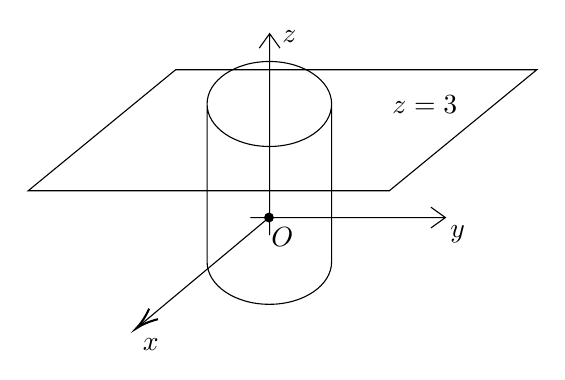
\begin{tikzpicture}[x=0.75pt,y=0.75pt,yscale=-1,xscale=1]
	\draw  (125.83,146.62) -- (219.83,146.62)(135.14,58) -- (135.14,155.06) (212.83,141.62) -- (219.83,146.62) -- (212.83,151.62) (130.14,65) -- (135.14,58) -- (140.14,65)  ;
	\draw  [fill={rgb, 255:red, 0; green, 0; blue, 0 }  ,fill opacity=1 ] (132.74,146.61) .. controls (132.74,145.45) and (133.68,144.52) .. (134.83,144.52) .. controls (135.98,144.52) and (136.91,145.45) .. (136.91,146.61) .. controls (136.91,147.76) and (135.98,148.69) .. (134.83,148.69) .. controls (133.68,148.69) and (132.74,147.76) .. (132.74,146.61) -- cycle ;
	\draw    (134.83,146.61) -- (72.36,198.78) ;
	\draw [shift={(70.83,200.06)}, rotate = 320.13] [color={rgb, 255:red, 0; green, 0; blue, 0 }  ][line width=0.75]    (10.93,-3.29) .. controls (6.95,-1.4) and (3.31,-0.3) .. (0,0) .. controls (3.31,0.3) and (6.95,1.4) .. (10.93,3.29)   ;
	\draw   (165,91.9) -- (165,167.95) .. controls (165,179.26) and (151.57,188.42) .. (135,188.42) .. controls (118.43,188.42) and (105,179.26) .. (105,167.95) -- (105,91.9)(165,91.9) .. controls (165,103.21) and (151.57,112.37) .. (135,112.37) .. controls (118.43,112.37) and (105,103.21) .. (105,91.9) .. controls (105,80.59) and (118.43,71.42) .. (135,71.42) .. controls (151.57,71.42) and (165,80.59) .. (165,91.9) -- cycle ;
	\draw   (89.83,75.42) -- (263.83,75.42) -- (192.83,133.69) -- (18.83,133.69) -- cycle ;
	\draw (221,149.4) node [anchor=north west][inner sep=0.75pt]    {$y$};
	\draw (140,55.4) node [anchor=north west][inner sep=0.75pt]    {$z$};
	\draw (134.74,150.01) node [anchor=north west][inner sep=0.75pt]    {$O$};
	\draw (72.83,203.46) node [anchor=north west][inner sep=0.75pt]    {$x$};
	\draw (193,86.4) node [anchor=north west][inner sep=0.75pt]    {$z=3$};
	\end{tikzpicture}
	\end{center}
	Those points form a circle in the hyperplane of $z=3$ centered at the point $(0,0,3)$ with a radius of $1$.
\end{eg}
\begin{thm}[Distance Formula in Three Dimension]
	For given points $P_1(x_1,y_1,z_1)$ and $P_2(x_2,y_2,z_2)$, the distance between them is denoted by $|P_1P_2|$ and is defined by \[|P_1P_2|=\sqrt{(x_1-x_2)^2+(y_1-y_2)^2+(z_1-z_2)^2}.\]	
\end{thm}
\begin{thm}[Equation of a Sphere]
	An equation of a sphere with a center of $(a,b,c)$ and a radius of $r$ is defined as \[(x-a)^2+(y-b)^2+(z-c)^2=r^2.\]	
\end{thm}
\begin{eg}
	What is the region in $\R^3$ represented by the inequalities \[1\leq x^2+y^2+z^2\leq4\quad\text{and}\quad z\leq0? \]	
	\begin{sol}
	\begin{center}
	\tikzset{every picture/.style={line width=0.75pt}}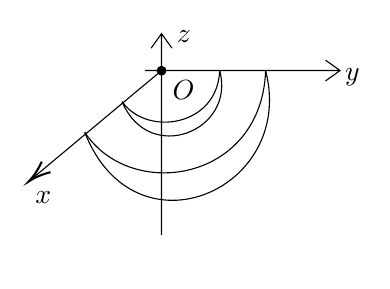
\begin{tikzpicture}[x=0.75pt,y=0.75pt,yscale=-1,xscale=1]
	\draw  (125.83,75.79) -- (219.83,75.79)(133.83,58) -- (133.83,155.06) (212.83,70.79) -- (219.83,75.79) -- (212.83,80.79) (128.83,65) -- (133.83,58) -- (138.83,65)  ;
	\draw  [fill={rgb, 255:red, 0; green, 0; blue, 0 }  ,fill opacity=1 ] (131.74,75.87) .. controls (131.74,74.72) and (132.68,73.79) .. (133.83,73.79) .. controls (134.98,73.79) and (135.91,74.72) .. (135.91,75.87) .. controls (135.91,77.02) and (134.98,77.96) .. (133.83,77.96) .. controls (132.68,77.96) and (131.74,77.02) .. (131.74,75.87) -- cycle ;
	\draw    (133.83,75.79) -- (71.36,127.96) ;
	\draw [shift={(69.83,129.24)}, rotate = 320.13] [color={rgb, 255:red, 0; green, 0; blue, 0 }  ][line width=0.75]    (10.93,-3.29) .. controls (6.95,-1.4) and (3.31,-0.3) .. (0,0) .. controls (3.31,0.3) and (6.95,1.4) .. (10.93,3.29)   ;
	\draw    (114.83,90.79) .. controls (126.83,107.79) and (160.83,102.79) .. (161.83,75.79) ;
	\draw    (114.83,90.79) .. controls (127.83,121.79) and (169.83,104.79) .. (161.83,75.79) ;
	\draw    (96.83,105.54) .. controls (119.08,139.26) and (182.11,129.34) .. (183.97,75.79) ;
	\draw    (96.83,105.54) .. controls (120.93,167.02) and (198.8,133.31) .. (183.97,75.79) ;
	\draw (221,73.4) node [anchor=north west][inner sep=0.75pt]    {$y$};
	\draw (140,55.4) node [anchor=north west][inner sep=0.75pt]    {$z$};
	\draw (137.91,79.27) node [anchor=north west][inner sep=0.75pt]    {$O$};
	\draw (71.83,132.64) node [anchor=north west][inner sep=0.75pt]    {$x$};
	\end{tikzpicture}
	\end{center}
	The region is the difference between the half spheres (the lower half of the sphere) centered at $(0,0,0)$ with a radius of $1$ and $2$.
	\end{sol}
\end{eg}

\subsection{Vectors}
\begin{df}[Vectors]
	\textbf{Vectors} are used to indicate a quantity that has both magnitude and direction. 
	\begin{center}
	\tikzset{every picture/.style={line width=0.75pt}}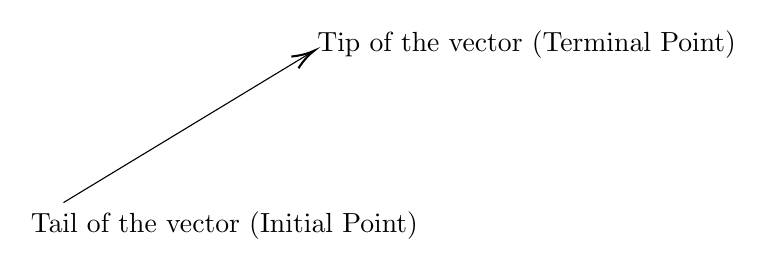
\begin{tikzpicture}[x=0.75pt,y=0.75pt,yscale=-1,xscale=1]
	\draw    (100,124) -- (219.12,51.82) ;
	\draw [shift={(220.83,50.79)}, rotate = 148.79] [color={rgb, 255:red, 0; green, 0; blue, 0 }  ][line width=0.75]    (10.93,-3.29) .. controls (6.95,-1.4) and (3.31,-0.3) .. (0,0) .. controls (3.31,0.3) and (6.95,1.4) .. (10.93,3.29)   ;
	\draw (83,127) node [anchor=north west][inner sep=0.75pt]   [align=left] {Tail of the vector (Initial Point)};
	\draw (221,40) node [anchor=north west][inner sep=0.75pt]   [align=left] {Tip of the vector (Terminal Point)};
	\end{tikzpicture}	
	\end{center}
	\begin{enumerate}
		\item Vectors are denoted as $\vec{v}.$
		\item Magnitude
		\begin{df}[Magnitude]
			A vector is a line segment, of which the \textbf{magnitude} of vector denoted by $|\vec{v}|$ is the length of it and the arrow points the direction of the vector. 
		\end{df}
	\end{enumerate}	
\end{df}
Vectors are operated in a different way: 
\begin{enumerate}
	\item Addition of Vectors: 
	\begin{enumerate}
		\item The triangle law: 
		\begin{center}
		\tikzset{every picture/.style={line width=0.75pt}}
		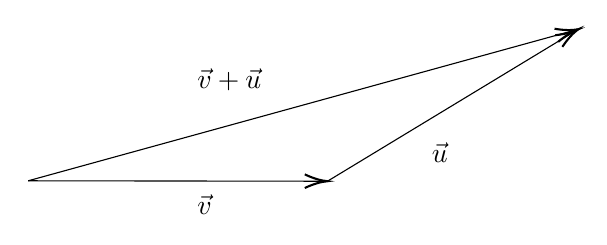
\begin{tikzpicture}[x=0.75pt,y=0.75pt,yscale=-1,xscale=1]
		\draw    (252,160) -- (371.12,87.82) ;
		\draw [shift={(372.83,86.79)}, rotate = 148.79] [color={rgb, 255:red, 0; green, 0; blue, 0 }  ][line width=0.75]    (10.93,-3.29) .. controls (6.95,-1.4) and (3.31,-0.3) .. (0,0) .. controls (3.31,0.3) and (6.95,1.4) .. (10.93,3.29)   ;
		\draw    (107.83,159.79) -- (250,160) ;
		\draw [shift={(252,160)}, rotate = 180.08] [color={rgb, 255:red, 0; green, 0; blue, 0 }  ][line width=0.75]    (10.93,-3.29) .. controls (6.95,-1.4) and (3.31,-0.3) .. (0,0) .. controls (3.31,0.3) and (6.95,1.4) .. (10.93,3.29)   ;
		\draw    (107.83,159.79) -- (370.9,87.32) ;
		\draw [shift={(372.83,86.79)}, rotate = 164.6] [color={rgb, 255:red, 0; green, 0; blue, 0 }  ][line width=0.75]    (10.93,-3.29) .. controls (6.95,-1.4) and (3.31,-0.3) .. (0,0) .. controls (3.31,0.3) and (6.95,1.4) .. (10.93,3.29)   ;
		\draw (188,165.4) node [anchor=north west][inner sep=0.75pt]    {$\vec{v}$};
		\draw (301,140.4) node [anchor=north west][inner sep=0.75pt]    {$\vec{u}$};
		\draw (188,104.4) node [anchor=north west][inner sep=0.75pt]    {$\vec{v} +\vec{u}$};
		\end{tikzpicture}	
		\end{center}
		\item The parallelogram law: 
		\begin{center}
		\tikzset{every picture/.style={line width=0.75pt}}
		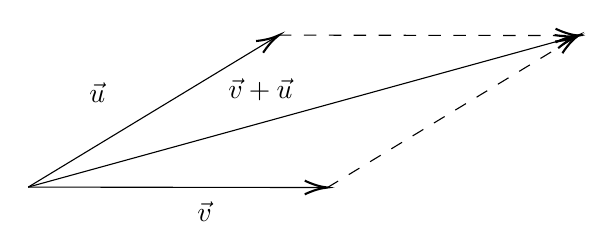
\begin{tikzpicture}[x=0.75pt,y=0.75pt,yscale=-1,xscale=1]
		\draw  [dash pattern={on 4.5pt off 4.5pt}]  (252,160) -- (371.12,87.82) ;
		\draw [shift={(372.83,86.79)}, rotate = 148.79] [color={rgb, 255:red, 0; green, 0; blue, 0 }  ][line width=0.75]    (10.93,-3.29) .. controls (6.95,-1.4) and (3.31,-0.3) .. (0,0) .. controls (3.31,0.3) and (6.95,1.4) .. (10.93,3.29)   ;
		\draw    (107.83,159.79) -- (250,160) ;
		\draw [shift={(252,160)}, rotate = 180.08] [color={rgb, 255:red, 0; green, 0; blue, 0 }  ][line width=0.75]    (10.93,-3.29) .. controls (6.95,-1.4) and (3.31,-0.3) .. (0,0) .. controls (3.31,0.3) and (6.95,1.4) .. (10.93,3.29)   ;
		\draw    (107.83,159.79) -- (370.9,87.32) ;
		\draw [shift={(372.83,86.79)}, rotate = 164.6] [color={rgb, 255:red, 0; green, 0; blue, 0 }  ][line width=0.75]    (10.93,-3.29) .. controls (6.95,-1.4) and (3.31,-0.3) .. (0,0) .. controls (3.31,0.3) and (6.95,1.4) .. (10.93,3.29)   ;
		\draw    (107.83,159.79) -- (226.95,87.61) ;
		\draw [shift={(228.66,86.57)}, rotate = 148.79] [color={rgb, 255:red, 0; green, 0; blue, 0 }  ][line width=0.75]    (10.93,-3.29) .. controls (6.95,-1.4) and (3.31,-0.3) .. (0,0) .. controls (3.31,0.3) and (6.95,1.4) .. (10.93,3.29)   ;
		\draw  [dash pattern={on 4.5pt off 4.5pt}]  (228.66,86.57) -- (370.83,86.78) ;
		\draw [shift={(372.83,86.79)}, rotate = 180.08] [color={rgb, 255:red, 0; green, 0; blue, 0 }  ][line width=0.75]    (10.93,-3.29) .. controls (6.95,-1.4) and (3.31,-0.3) .. (0,0) .. controls (3.31,0.3) and (6.95,1.4) .. (10.93,3.29)   ;
		\draw (188,165.4) node [anchor=north west][inner sep=0.75pt]    {$\vec{v}$};
		\draw (136,108.4) node [anchor=north west][inner sep=0.75pt]    {$\vec{u}$};
		\draw (203,106.4) node [anchor=north west][inner sep=0.75pt]    {$\vec{v} +\vec{u}$};
		\end{tikzpicture}
		\end{center}
	\end{enumerate}
	\item Scalar Multiplications: 
	\begin{center}
	\tikzset{every picture/.style={line width=0.75pt}}
	\begin{tikzpicture}[x=0.75pt,y=0.75pt,yscale=-1,xscale=1]
	\draw    (237.83,126.79) -- (349.03,72.66) ;
	\draw [shift={(350.83,71.79)}, rotate = 154.05] [color={rgb, 255:red, 0; green, 0; blue, 0 }  ][line width=0.75]    (10.93,-3.29) .. controls (6.95,-1.4) and (3.31,-0.3) .. (0,0) .. controls (3.31,0.3) and (6.95,1.4) .. (10.93,3.29)   ;
	\draw [color={rgb, 255:red, 128; green, 128; blue, 128 }  ,draw opacity=1 ]   (237.83,126.79) -- (126.63,180.91) ;
	\draw [shift={(124.83,181.79)}, rotate = 334.05] [color={rgb, 255:red, 128; green, 128; blue, 128 }  ,draw opacity=1 ][line width=0.75]    (10.93,-3.29) .. controls (6.95,-1.4) and (3.31,-0.3) .. (0,0) .. controls (3.31,0.3) and (6.95,1.4) .. (10.93,3.29)   ;
	\draw    (237.83,126.79) -- (292.53,100.16) ;
	\draw [shift={(294.33,99.29)}, rotate = 154.05] [color={rgb, 255:red, 0; green, 0; blue, 0 }  ][line width=0.75]    (10.93,-3.29) .. controls (6.95,-1.4) and (3.31,-0.3) .. (0,0) .. controls (3.31,0.3) and (6.95,1.4) .. (10.93,3.29)   ;
	\draw (352.83,75.19) node [anchor=north west][inner sep=0.75pt]    {$\vec{v}$};
	\draw (166.83,164.19) node [anchor=north west][inner sep=0.75pt]    {$-\vec{v}$};
	\draw (268.08,116.44) node [anchor=north west][inner sep=0.75pt]    {$\frac{1}{2}\vec{v}$};
	\end{tikzpicture}
	\end{center}
	\begin{df}[Scalar Multiplication]
		If $c\in\R$ and $\vec{v}$ is a vector, then $c\vec{v}$ is in the same direction of $\vec{v}$ if $c>0$ and in the opposite direction if $c<0$.
	\end{df}
	\begin{thm}
		The magnitude of $c\vec{v}$: \[|c\vec{v}|=c|\vec{v}|.\]
	\end{thm}
	\item Differences of Vectors: 
	\begin{center}
		\tikzset{every picture/.style={line width=0.75pt}}
	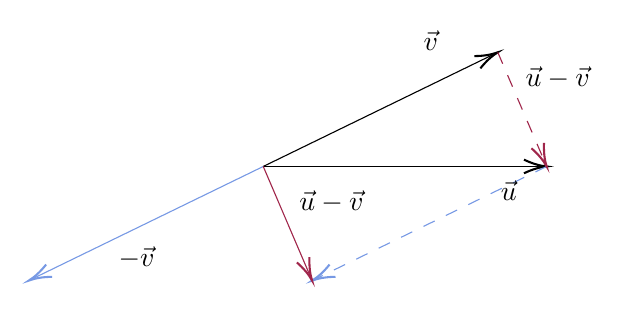
\begin{tikzpicture}[x=0.75pt,y=0.75pt,yscale=-1,xscale=1]
	\draw    (237.83,126.79) -- (349.03,72.66) ;
	\draw [shift={(350.83,71.79)}, rotate = 154.05] [color={rgb, 255:red, 0; green, 0; blue, 0 }  ][line width=0.75]    (10.93,-3.29) .. controls (6.95,-1.4) and (3.31,-0.3) .. (0,0) .. controls (3.31,0.3) and (6.95,1.4) .. (10.93,3.29)   ;
	\draw [color={rgb, 255:red, 155; green, 155; blue, 155 }  ,draw opacity=1 ]   (237.83,126.79) -- (126.63,180.91) ;
	\draw [shift={(124.83,181.79)}, rotate = 334.05] [color={rgb, 255:red, 155; green, 155; blue, 155 }  ,draw opacity=1 ][line width=0.75]    (10.93,-3.29) .. controls (6.95,-1.4) and (3.31,-0.3) .. (0,0) .. controls (3.31,0.3) and (6.95,1.4) .. (10.93,3.29)   ;
	\draw    (237.83,126.79) -- (372.37,126.79) ;
	\draw [shift={(374.37,126.79)}, rotate = 180] [color={rgb, 255:red, 0; green, 0; blue, 0 }  ][line width=0.75]    (10.93,-3.29) .. controls (6.95,-1.4) and (3.31,-0.3) .. (0,0) .. controls (3.31,0.3) and (6.95,1.4) .. (10.93,3.29)   ;
	\draw [color={rgb, 255:red, 155; green, 155; blue, 155 }  ,draw opacity=1 ] [dash pattern={on 4.5pt off 4.5pt}]  (374.37,126.79) -- (263.17,180.91) ;
	\draw [shift={(261.37,181.79)}, rotate = 334.05] [color={rgb, 255:red, 155; green, 155; blue, 155 }  ,draw opacity=1 ][line width=0.75]    (10.93,-3.29) .. controls (6.95,-1.4) and (3.31,-0.3) .. (0,0) .. controls (3.31,0.3) and (6.95,1.4) .. (10.93,3.29)   ;
	\draw [color={rgb, 255:red, 208; green, 2; blue, 27 }  ,draw opacity=1 ]   (237.83,126.79) -- (260.59,179.95) ;
	\draw [shift={(261.37,181.79)}, rotate = 246.82] [color={rgb, 255:red, 208; green, 2; blue, 27 }  ,draw opacity=1 ][line width=0.75]    (10.93,-3.29) .. controls (6.95,-1.4) and (3.31,-0.3) .. (0,0) .. controls (3.31,0.3) and (6.95,1.4) .. (10.93,3.29)   ;
	\draw [color={rgb, 255:red, 208; green, 2; blue, 27 }  ,draw opacity=1 ] [dash pattern={on 4.5pt off 4.5pt}]  (350.83,71.79) -- (373.59,124.95) ;
	\draw [shift={(374.37,126.79)}, rotate = 246.82] [color={rgb, 255:red, 208; green, 2; blue, 27 }  ,draw opacity=1 ][line width=0.75]    (10.93,-3.29) .. controls (6.95,-1.4) and (3.31,-0.3) .. (0,0) .. controls (3.31,0.3) and (6.95,1.4) .. (10.93,3.29)   ;
	\draw (313.83,60.19) node [anchor=north west][inner sep=0.75pt]    {$\vec{v}$};
	\draw (166.83,164.19) node [anchor=north west][inner sep=0.75pt]    {$-\vec{v}$};
	\draw (351,132.4) node [anchor=north west][inner sep=0.75pt]    {$\vec{u}$};
	\draw (254,137.4) node [anchor=north west][inner sep=0.75pt]    {$\vec{u} -\vec{v}$};
	\draw (363,77.4) node [anchor=north west][inner sep=0.75pt]    {$\vec{u} -\vec{v}$};
	\end{tikzpicture}
	\end{center}
 	The difference of vectors $\vecu$ and $\vecv$ is denoted by $\vecu-\vecv$ and is defined by \[\vecu-\vecv=\vecu+(-\vecv)\]
 	\item Properties of vectors: \\Suppose $\veca,\ \vecb,\ \vecc$ are vectors in $V_n$ and $c$ and $d$ are scalars (\textit{Those properties can be proven geometrically}): 
 	\begin{enumerate}
 		\item $\veca+\vecb=\vecb+\veca$
 		\item $\veca+(\vecb+\vecc)=(\veca+\vecb)+\vecc$
 		\item $\veca+0=\veca$
 		\item $\veca+(-\veca)=0$
 		\item $c(\veca+\vecb)=c\veca+c\vecb$
 		\item $(c+d)\veca=c\veca+d\veca$
 		\item $(cd)\veca=c(d\veca)$
 		\item $1\cdot\veca=\veca$
 	\end{enumerate}
\end{enumerate}
We can link the coordinate system and vectors together:  
\begin{enumerate}
	\item \begin{df}[Components of Vectors] We will denote vector $\vecv$ as \[\vecv=\langle a_1,a_2\rangle,\] where $a_1$ and $a_2$ are called the \textbf{components} of $\vecv.$ \end{df}
	\begin{center}
	\tikzset{every picture/.style={line width=0.75pt}} 
	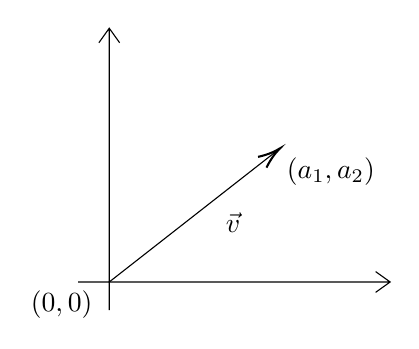
\begin{tikzpicture}[x=0.75pt,y=0.75pt,yscale=-1,xscale=1]
	\draw  (50,191.25) -- (200.37,191.25)(65.04,69) -- (65.04,204.83) (193.37,186.25) -- (200.37,191.25) -- (193.37,196.25) (60.04,76) -- (65.04,69) -- (70.04,76)  ;
	\draw    (65.04,191.25) -- (145.8,128.06) ;
	\draw [shift={(147.37,126.83)}, rotate = 141.96] [color={rgb, 255:red, 0; green, 0; blue, 0 }  ][line width=0.75]    (10.93,-3.29) .. controls (6.95,-1.4) and (3.31,-0.3) .. (0,0) .. controls (3.31,0.3) and (6.95,1.4) .. (10.93,3.29)   ;
	\draw (26,194.4) node [anchor=north west][inner sep=0.75pt]    {$( 0,0)$};
	\draw (149.37,130.23) node [anchor=north west][inner sep=0.75pt]    {$( a_{1} ,a_{2})$};
	\draw (120,156.4) node [anchor=north west][inner sep=0.75pt]    {$\vec{v}$};
	\end{tikzpicture}
	\end{center}
	\item In the three dimension: \[\vecv=\langle a_1,a_2,a_3\rangle\]
	\begin{center}
	\tikzset{every picture/.style={line width=0.75pt}}
	\begin{tikzpicture}[x=0.75pt,y=0.75pt,yscale=-1,xscale=1]
	\draw  (131,163.25) -- (281.37,163.25)(146.04,41) -- (146.04,176.83) (274.37,158.25) -- (281.37,163.25) -- (274.37,168.25) (141.04,48) -- (146.04,41) -- (151.04,48)  ;
	\draw    (146.04,163.25) -- (226.8,100.06) ;
	\draw [shift={(228.37,98.83)}, rotate = 141.96] [color={rgb, 255:red, 0; green, 0; blue, 0 }  ][line width=0.75]    (10.93,-3.29) .. controls (6.95,-1.4) and (3.31,-0.3) .. (0,0) .. controls (3.31,0.3) and (6.95,1.4) .. (10.93,3.29)   ;
	\draw    (146.04,163.25) -- (88.61,236.53) ;
	\draw [shift={(87.37,238.1)}, rotate = 308.09] [color={rgb, 255:red, 0; green, 0; blue, 0 }  ][line width=0.75]    (10.93,-3.29) .. controls (6.95,-1.4) and (3.31,-0.3) .. (0,0) .. controls (3.31,0.3) and (6.95,1.4) .. (10.93,3.29)   ;
	\draw (90,144.4) node [anchor=north west][inner sep=0.75pt]    {$( 0,0,0)$};
	\draw (230.37,102.23) node [anchor=north west][inner sep=0.75pt]    {$( a_{1} ,a_{2} ,a_{3})$};
	\draw (201,128.4) node [anchor=north west][inner sep=0.75pt]    {$\vec{v}$};
	\draw (97,236.4) node [anchor=north west][inner sep=0.75pt]    {$x$};
	\draw (281,169.4) node [anchor=north west][inner sep=0.75pt]    {$y$};
	\draw (127,40.4) node [anchor=north west][inner sep=0.75pt]    {$z$};
	\end{tikzpicture}
	\end{center}
	\item \begin{df} If $A(x_1,y_1,z_1)$ as the tail of vector $\vecv$ and $B(x_1,y_1,z_1)$ as the tip of vector $\vecv$, then \[\overrightarrow{AB}=\langle x_2-x_1,\ y_2-y_1,\ z_2-z_1\rangle\]\[|\overrightarrow{AB}|=\sqrt{(x_2-x_1)^2+(y_2-y_1)^2+(z_2-z_1)^2}\]\end{df}
	\item \begin{thm}If $\vecv=\langle a,b,c\rangle$ and $\vecu=\langle a',b',c'\rangle$, then \[\vecu+\vecv=\langle a'+a,\ b'+b,\ c'+c\rangle\]\[\vecu-\vecv=\langle a'-a,\ b'-b,\ c'-c\rangle\]\[\alpha\vecu=\langle\alpha a',\ \alpha b',\ \alpha c'\rangle,\text{ where }\alpha\text{ is a scalar.}\]\end{thm}
\end{enumerate}

\begin{df}[Standard Basis Vectors]
	In 2-D, $\veci=\langle 1,0\rangle$ and $\vecj=\langle0,1\rangle$; and in 3-D, $\veci=\langle1,0,0\rangle$, $\vecj=\langle0,1,0\rangle$, and $\veck=\langle0,0,1\rangle$ are called the \textbf{standard basis vectors}. 
	\begin{rmk} Any vectors in 2D and 3D can be written as \[\vecv=\langle a,b,c\rangle=a\veci+b\vecj+c\veck.\]\end{rmk}
\end{df}
\begin{df}[Unit Vector]
	A \textbf{unit vector}is a vector of magnitude of $1$. 
	\begin{eg} \[|\veci|=|\vecj|=|\veck|=1\text{ are unit vectors.}\]\end{eg}
	\begin{thm}
		To find a unit vector in the direction of any vector $\vecv$, we use $\displaystyle\frac{1}{|\vecv|}\vecv$. The length of vector $\displaystyle\frac{\vecv}{|\vecv|}$ is $1$ and its direction is the same as $\vecv$.	
	\end{thm}
\end{df}
\begin{eg}
	If the vectors in the figure satisfy $|\vecu|=|\vecv|=1$, and $\vecu+\vecv+\vecw=0$, find $|\vecw|$.
	\begin{center}
	\tikzset{every picture/.style={line width=0.75pt}}
	\begin{tikzpicture}[x=0.75pt,y=0.75pt,yscale=-1,xscale=1]
	\draw    (100,136.1) -- (222.37,136.1) ;
	\draw [shift={(224.37,136.1)}, rotate = 180] [color={rgb, 255:red, 0; green, 0; blue, 0 }  ][line width=0.75]    (10.93,-3.29) .. controls (6.95,-1.4) and (3.31,-0.3) .. (0,0) .. controls (3.31,0.3) and (6.95,1.4) .. (10.93,3.29)   ;
	\draw    (100,136.1) -- (51.89,87.99) ;
	\draw [shift={(50.47,86.57)}, rotate = 45] [color={rgb, 255:red, 0; green, 0; blue, 0 }  ][line width=0.75]    (10.93,-3.29) .. controls (6.95,-1.4) and (3.31,-0.3) .. (0,0) .. controls (3.31,0.3) and (6.95,1.4) .. (10.93,3.29)   ;
	\draw    (100,136.1) -- (52.79,183.31) ;
	\draw [shift={(51.37,184.73)}, rotate = 315] [color={rgb, 255:red, 0; green, 0; blue, 0 }  ][line width=0.75]    (10.93,-3.29) .. controls (6.95,-1.4) and (3.31,-0.3) .. (0,0) .. controls (3.31,0.3) and (6.95,1.4) .. (10.93,3.29)   ;
	\draw   (85.66,136.16) -- (92.8,128.96) -- (100,136.1) -- (92.86,143.3) -- cycle ;
	\draw (61,75.4) node [anchor=north west][inner sep=0.75pt]    {$\vec{u}$};
	\draw (67,174.4) node [anchor=north west][inner sep=0.75pt]    {$\vec{v}$};
	\draw (204,143.4) node [anchor=north west][inner sep=0.75pt]    {$\vec{w}$};
	\end{tikzpicture}
	\end{center}
	\begin{sol}
	Decompose the vectors: 
	\begin{center}
	\tikzset{every picture/.style={line width=0.75pt}} 
	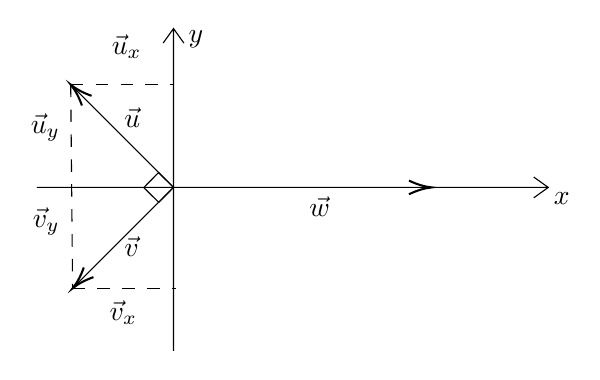
\begin{tikzpicture}[x=0.75pt,y=0.75pt,yscale=-1,xscale=1]
	\draw    (100,136.1) -- (222.37,136.1) ;
	\draw [shift={(224.37,136.1)}, rotate = 180] [color={rgb, 255:red, 0; green, 0; blue, 0 }  ][line width=0.75]    (10.93,-3.29) .. controls (6.95,-1.4) and (3.31,-0.3) .. (0,0) .. controls (3.31,0.3) and (6.95,1.4) .. (10.93,3.29)   ;
	\draw    (100,136.1) -- (51.89,87.99) ;
	\draw [shift={(50.47,86.57)}, rotate = 45] [color={rgb, 255:red, 0; green, 0; blue, 0 }  ][line width=0.75]    (10.93,-3.29) .. controls (6.95,-1.4) and (3.31,-0.3) .. (0,0) .. controls (3.31,0.3) and (6.95,1.4) .. (10.93,3.29)   ;
	\draw    (100,136.1) -- (52.79,183.31) ;
	\draw [shift={(51.37,184.73)}, rotate = 315] [color={rgb, 255:red, 0; green, 0; blue, 0 }  ][line width=0.75]    (10.93,-3.29) .. controls (6.95,-1.4) and (3.31,-0.3) .. (0,0) .. controls (3.31,0.3) and (6.95,1.4) .. (10.93,3.29)   ;
	\draw   (85.66,136.16) -- (92.8,128.96) -- (100,136.1) -- (92.86,143.3) -- cycle ;
	\draw  (34.17,136.1) -- (280.55,136.1)(100,59.56) -- (100,214.82) (273.55,131.1) -- (280.55,136.1) -- (273.55,141.1) (95,66.56) -- (100,59.56) -- (105,66.56)  ;
	\draw  [dash pattern={on 4.5pt off 4.5pt}]  (50.47,86.57) -- (100.37,86.57) ;
	\draw  [dash pattern={on 4.5pt off 4.5pt}]  (50.47,86.57) -- (51.37,184.73) ;
	\draw  [dash pattern={on 4.5pt off 4.5pt}]  (51.37,184.73) -- (101.28,184.73) ;
	\draw (75,96.4) node [anchor=north west][inner sep=0.75pt]    {$\vec{u}$};
	\draw (75,158.4) node [anchor=north west][inner sep=0.75pt]    {$\vec{v}$};
	\draw (164.19,139.5) node [anchor=north west][inner sep=0.75pt]    {$\vec{w}$};
	\draw (282,137.4) node [anchor=north west][inner sep=0.75pt]    {$x$};
	\draw (106,59.4) node [anchor=north west][inner sep=0.75pt]    {$y$};
	\draw (30,99.4) node [anchor=north west][inner sep=0.75pt]    {$\vec{u}_{y}$};
	\draw (31,144.4) node [anchor=north west][inner sep=0.75pt]    {$\vec{v}_{y}$};
	\draw (69,61.4) node [anchor=north west][inner sep=0.75pt]    {$\vec{u}_{x}$};
	\draw (68,189.4) node [anchor=north west][inner sep=0.75pt]    {$\vec{v}_{x}$};
	\end{tikzpicture}
	\end{center}
	We then have \[\cos{45^\circ}=\frac{|\vecu_x|}{\vecu}\Longrightarrow|\vecu_x|=|\vecu|\cos{45^\circ}; \] \[\sin{45^\circ}=\frac{|\vecu_y|}{\vecu}\Longrightarrow|\vecu_y|=|\vecu|\sin{45^\circ}; \]
	\[\begin{aligned}
		\therefore \vecu=\langle|\vecu_x|,\ |\vecu_y\rangle&=-|\vecu_x|\veci+|\vecu_y|\vecj\\
		&=-\frac{\sqrt{2}}{2}|\vecu|\veci+\frac{\sqrt{2}}{2}\vecj\\
		&=\frac{\sqrt{2}}{2}|\vecu|(-\veci+\vecj)
	\end{aligned}\]
	Similarly, \[\vecv=\frac{\sqrt{2}}{2}|\vecv|(-\veci-\vecj).\]
	We know $\vecu+\vecv+\vecw=0$: \[\therefore\vecw+\frac{\sqrt{2}}{2}|\vecu|(-\veci+\vecj)+\frac{\sqrt{2}}{2}|\vecv|(-\veci-\vecj)=0\]
	We know $|\vecu|=|\vecv|=1$: \[\begin{aligned}
		\therefore \vecw+\frac{\sqrt{2}}{2}(-\veci+\vecj)+\frac{\sqrt{2}}{2}(-\veci-\vecj)&=0\\
		\vecw+\frac{\sqrt{2}}{2}(-\veci+\vecj-\veci-\vecj)&=0\\
		\vecw&=\sqrt{2}\veci
	\end{aligned}\]
	\[\therefore \vecw=\langle\sqrt{2},0\rangle\Longrightarrow|\vecw|=\sqrt{2}.\]
	\end{sol}
\end{eg}

\subsection{Dot Product}
\begin{df}[Dot Product]
	If $\vecu=\langle x_1,y_1,z_1\rangle$ and $\vecv=\langle x_2,y_2,z_2\rangle$, then the dot product of $\vecu$ and $\vecv$ is defined as \[\begin{aligned}
		\vecu\cdot\vecv&=\langle x_1,y_1,z_1\rangle\cdot\langle x_2,y_2,z_2\rangle\\
		&=x_1x_2+y_1y_1+z_1z_2 
	\end{aligned}\]	
	\begin{rmk} The dot product of two vectors returns a scalar. \end{rmk}
	\begin{eg}
		Let $\vecu=\veci+2\vecj-3\veck$ and $\vecv=2\vecj-\veck$. Find $\vecu\cdot\vecv$.\\
		\begin{sol}
			\[\begin{aligned}
			\vecu\cdot\vecv&=\langle1,2,-3\rangle\cdot\langle0,2,-1\rangle\\
				&=(1)(0)+(2)(2)+(-3)(-1)=7.
			\end{aligned}\]	
		\end{sol}
	\end{eg}
\end{df}
Properties of the dot product: 
\begin{enumerate}
	\item $\veca\cdot\vecb=\vecb\cdot\veca$
	\item $\veca\cdot(\vecv+\vecc)=\veca\vecb+\veca\vecc$
	\item $m(\veca\cdot\vecb)=(m\veca)\cdot\vecb=\veca\cdot(m\vecb)=(\veca\cdot\vecb)m$
	\item $\veci\cdot\veci=\vecj\cdot\vecj=\veck\cdot\veck=1$\\$\veci\cdot\vecj=\vecj\cdot\veck=\veck\cdot\veci=0$
\end{enumerate}
\begin{thm}
	\[\vecu\cdot\vecu=|\vecu|^2.\]	
\end{thm}
\begin{thm}
	If $\theta$ is the angle between $\vecu$ and $\vecv$, then \[\boxed{\vecu\cdot\vecv=|\vecu|\cdot|\vecv|\cos\theta}.\]
	\begin{ext} \[\cos\theta=\frac{\vecu\cdot\vecv}{|\vecu||\vecv|}\]\end{ext}
	\begin{ext} \[\theta=90^\circ\Longleftrightarrow\vecu\cdot\vecv=0.\]	\end{ext}
\end{thm}
\begin{df}[Projections]
	We use $\Proj_{\veca}\vecb$ to denote the \textbf{projection} of $\vecb$ on $\veca$.
	\begin{center}
	\tikzset{every picture/.style={line width=0.75pt}}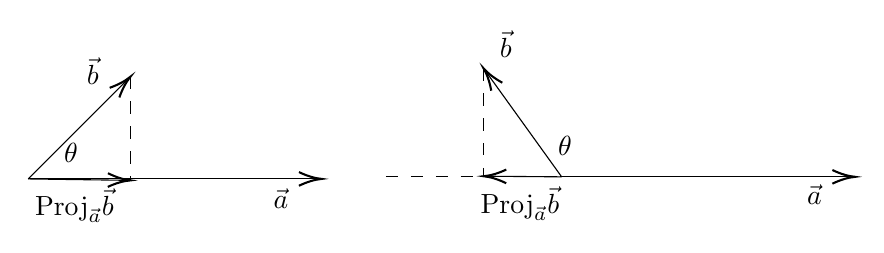
\begin{tikzpicture}[x=0.75pt,y=0.75pt,yscale=-1,xscale=1]
	\draw    (100,118) -- (239.37,118) ;
	\draw [shift={(241.37,118)}, rotate = 180] [color={rgb, 255:red, 0; green, 0; blue, 0 }  ][line width=0.75]    (10.93,-3.29) .. controls (6.95,-1.4) and (3.31,-0.3) .. (0,0) .. controls (3.31,0.3) and (6.95,1.4) .. (10.93,3.29)   ;
	\draw    (100,118) -- (147.89,70.11) ;
	\draw [shift={(149.3,68.7)}, rotate = 135] [color={rgb, 255:red, 0; green, 0; blue, 0 }  ][line width=0.75]    (10.93,-3.29) .. controls (6.95,-1.4) and (3.31,-0.3) .. (0,0) .. controls (3.31,0.3) and (6.95,1.4) .. (10.93,3.29)   ;
	\draw    (357,117) -- (496.37,117) ;
	\draw [shift={(498.37,117)}, rotate = 180] [color={rgb, 255:red, 0; green, 0; blue, 0 }  ][line width=0.75]    (10.93,-3.29) .. controls (6.95,-1.4) and (3.31,-0.3) .. (0,0) .. controls (3.31,0.3) and (6.95,1.4) .. (10.93,3.29)   ;
	\draw    (357,117) -- (320.54,66.32) ;
	\draw [shift={(319.37,64.7)}, rotate = 54.27] [color={rgb, 255:red, 0; green, 0; blue, 0 }  ][line width=0.75]    (10.93,-3.29) .. controls (6.95,-1.4) and (3.31,-0.3) .. (0,0) .. controls (3.31,0.3) and (6.95,1.4) .. (10.93,3.29)   ;
	\draw    (100,118) -- (147.3,118.67) ;
	\draw [shift={(149.3,118.7)}, rotate = 180.81] [color={rgb, 255:red, 0; green, 0; blue, 0 }  ][line width=0.75]    (10.93,-3.29) .. controls (6.95,-1.4) and (3.31,-0.3) .. (0,0) .. controls (3.31,0.3) and (6.95,1.4) .. (10.93,3.29)   ;
	\draw  [dash pattern={on 4.5pt off 4.5pt}]  (149.3,68.7) -- (149.3,118.7) ;
	\draw  [dash pattern={on 4.5pt off 4.5pt}]  (272.37,117) -- (357,117) ;
	\draw  [dash pattern={on 4.5pt off 4.5pt}]  (319.37,64.7) -- (319.37,116.7) ;
	\draw    (357,117) -- (321.37,116.71) ;
	\draw [shift={(319.37,116.7)}, rotate = 0.46] [color={rgb, 255:red, 0; green, 0; blue, 0 }  ][line width=0.75]    (10.93,-3.29) .. controls (6.95,-1.4) and (3.31,-0.3) .. (0,0) .. controls (3.31,0.3) and (6.95,1.4) .. (10.93,3.29)   ;
	\draw (116,99.4) node [anchor=north west][inner sep=0.75pt]    {$\theta $};
	\draw (354,96.4) node [anchor=north west][inner sep=0.75pt]    {$\theta $};
	\draw (217,121.4) node [anchor=north west][inner sep=0.75pt]    {$\vec{a}$};
	\draw (474,119.4) node [anchor=north west][inner sep=0.75pt]    {$\vec{a}$};
	\draw (127,58.4) node [anchor=north west][inner sep=0.75pt]    {$\vec{b}$};
	\draw (326,45.4) node [anchor=north west][inner sep=0.75pt]    {$\vec{b}$};
	\draw (102,121.4) node [anchor=north west][inner sep=0.75pt]    {$\Proj_{\vec{a}}\vec{b}$};
	\draw (316.69,120.4) node [anchor=north west][inner sep=0.75pt]    {$\Proj_{\vec{a}}\vec{b}$};
	\end{tikzpicture}
	\end{center}
	From the diagrams, \[\cos\theta=\frac{|\Proj_{\veca}\vecb|}{|\vecb|}\Longrightarrow|\Proj_{\veca}\vecb=\boxed{|\vecb|\cos\theta}.\]
	We know that \[\begin{aligned}
		\veca\cdot\vecb&=|\veca||\vecb|\cos\theta\\
		\therefore\frac{\veca\cdot\vecb}{|\veca|}&=\boxed{|\vecb|\cos\theta}\\
		\therefore |\Proj_{\veca}\vecb|&=\frac{\veca\cdot\vecb}{|\veca|},\text{ which is a scalar.}
	\end{aligned}\]
	$|\Proj_{\veca}\vecb|$ is called the \textbf{scalar projection} of $\vecb$ on $\veca$.
	\[\Proj_{\veca}\vecb=|\Proj_{\veca}\vecb|\cdot\underbrace{\frac{\veca}{|\veca|}}_{\text{unit vector}}=\frac{\veca\cdot\vecb}{|\veca|}\cdot\frac{\veca}{|\veca|}=\frac{\veca\cdot\vecb}{|\veca|^2}\cdot\veca\]
	$\Proj_{\veca}\vecb$ is called \textbf{projection} of $\vecb$ on $\veca$ and is a vector. 
\end{df}







\end{document}